\chapter{Detección con Aprendizaje Profundo}\label{cap.deteccion}
En este capítulo se realizará una primera aproximación al problema de la detección mediante el aprendizaje profundo utilizando la misma plataforma que se ha estado empleando hasta el momento, Caffe. Para ello se ha utilizado la rama \textit{\acrfull{ssd}}~\cite{liu2016ssd}de la misma, que, además de permitir el entrenamiento de modelos para la detección de diferentes objetos en función de la base de datos utilizada, ofrece varios modelos que ya han sido entrenados para facilitar esta tarea.\\

El método utilizado, \acrshort{ssd}, es diseñado para detectar objetos en imágenes utilizando una única red neuronal profunda. El enfoque \acrshort{ssd} se basa en una red convolucional \textit{feed-forward} que produce una colección de tamaño fijo de cajas delimitadoras(\textit{bounding boxes}) y puntuaciones para la presencia de instancias de clase de objetos en esas cajas, seguido de un paso de supresión no máxima para producir las detecciones finales. Las primeras capas de red se basan en una arquitectura estándar utilizada para la clasificación de imágenes de alta calidad (truncada antes de cualquier clasificación), similar a la explicada en el Capítulo~\ref{cap.clasificacion}. Posteriormente se añade una estructura auxiliar a la red para producir las detecciones, teniendo en cuenta una serie de características clave:
\begin{itemize}
	\item \textbf{Mapas de características de múltiples escalas para detección.} Se añaden capas de características convolucionales al final de la red base truncada, cuyyo tamaño disminuye progresivamente, permitiendo predicciones de detecciones a múltiple escalas. El modelo convolucional para la predicción de las detecciones es diferente para cada capa característica.
	\vspace{10pt}
	\item \textbf{Predictores convolucionales para la detección.} Cada capa de característica añadida puede producir un conjunto fijo de predicciones de detección usando un conjunto de filtros convolucionales, que son indicados en la parte superior de la arquitectura de red \acrshort{ssd}.
	\item \textbf{Cajas por defecto y relaciones de aspecto.} Se asocia un conjunto de cajas delimitadoras predeterminadas con cada celda de mapa de carcaterísticas, para varios mapas de características en la parte superior de la red. Las cajas por defecto anidan el mapa de características de una manera convolucional, de modo que la posición de cada caja con respecto a su celda correspondiente es fija. En cada celda de mapa de características, se predicen los desplazamientos relativos a las formas de cajas predeterminadas en la celda, así como las puntuaciones por clase que indican la presencia de una instancia de clase en cada uno de esas cajas.
\end{itemize}

En la Figura~\ref{fig.ssd} se muestra un resumen del funcionamiento de este modelo. \acrshort{ssd} sólo necesita una imagen de entrada y cajas de verdad para cada objeto durante el entrenamiento. De forma convolucional, se evalua un conjunto pequeño de cajas predeterminadas de diferentes relaciones de aspecto en cada ubicación en varios mapas de características con diferentes escalas (por ejemplo, $8\times8$ en~(b) y $4\times4$ en~(c)). Para cada caja predeterminada se predice tanto los desplazamientos de forma como las confidencias para todas las categorías de objetos (($c_1, c_2, ... , c_p)$). En el momento del entrenamiento, primero se coincide con estas cajas por defecto las casillas de verdad.

\begin{figure}[H]
	\begin{center}
		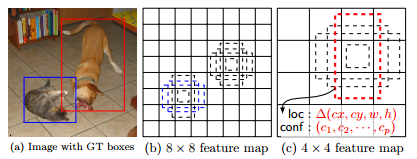
\includegraphics[width=0.6\textwidth]{figures/ssd}
		\caption{Modelo \acrshort{ssd}. Imagen obtenida de~\cite{2015arXiv151202325L}}
		\label{fig.ssd}
	\end{center}
\end{figure} 

Durante el entrenamiento es necesario determinar qué casillas por defecto corresponden a una detección de verdad y entrenar la red en consecuencia. Se comienza haciendo coincidir cada caja de verdad con la caja predeterminada con la mejor superposición de \textit{Jaccard}, un estadístico utilizado para comparar la similitud y diversidad de conjuntos de muestras. 
Esto simplifica el problema de aprendizaje, permitiendo a la red predecir puntuaciones altas para múltiples cajas por defecto superpuestas en lugar de requerir que elija sólo la que tenga superposición máxima. Tras el paso de la coincidencia, la mayoría de las cajas predeterminadas son negativas, especialmente cuando el número de cajas predeterminadas posibles es grande, introduciendo un desequilibrio significativo entre los ejemplos de entrenamiento positivos y negativos. Poe ello es necesario realizar una minería negativa dura, de tal manera que, en lugar de usar todos los ejemplos negativos, se clasifican usando la pérdida de confianza más alta para cada caja predeterminada y se seleccionan los más altos para que la relación entre los negativos y los positivos sea como mucho 3:1, conduciendo a una optimización más rápida y un entrenamiento más estable. Pr último, para hacer que el modelo sea más robusto a los diferentes tamaños y formas de los objetos de entrada, cada imagen de entrenamiento se muestreará aleatoriamente mediante el uso de toda la imagen de entrada original, el muestreo de un parche de modo que la superposición mínima de jaccard con los objetos sea de 0.1, 0.3,
0.5, 0.7 o 0.9, o el muestreo al azar un parche.\\

Una vez entendido el funcionamiento de las redes \acrshort{ssd}, cuya información ha sido obtenida de~\cite{2015arXiv151202325L}, se pasará al uso de algunos ejemplos de las mismas, proporcionadas por la propia rama de la plataforma Caffe. El motivo del uso de estos modelos ya entrenados viene dado por la alta capacidad de cómputo necesaria para entrenar este tipo de redes y la el tiempo que implica el entrenamiento. En concreto se analizarán algunas imágenes con dos de las redes \acrshort{ssd} que se proporcionan:
\begin{itemize}
	\item \textbf{VOC0712-SSD300x300.} Este modelo ha sido entrenado con las bases de datos \textit{Pascal VOC} de los años 2007~\cite{pascal-voc-2007} y 2012~\cite{pascal-voc-2012}, explicadas en la Sección~\ref{sec.voc}. Se utilizan imágenes de 300x300 y la red formada en la iteración 120000.
	\item \textbf{COCO-SSD300x300} Este modelo ha sido entrenado con las bases de datos \acrshort{coco}, explicadas en la Sección~\ref{sec.coco}. Se utilizan imágenes de 300x300 y la red formada en la iteración 120000.
\end{itemize}

Estos modelos proporcionados por la rama \acrshort{ssd} de Caffe pueden ser descargados de su repositorio \textit{Git Hub}~\footnote{https://github.com/weiliu89/caffe/tree/ssd} y utilizados para desarrollar la aplicación que sea de interés.\\

Al obtener los modelos se encuentra una carpeta con una serie de archivos que permiten comprobar la estructura de la red, el solucionador o el propio modelo entrenado entre otros. La aplicación de interés, se centra en el uso de tres de los archivos proporcionados:
\begin{itemize}
	\item \textbf{\textit{labelmap\_voc.prototxt}}, contiene la estructura de las diferentes etiquetas que pueden ser asignadas.
	\item \textbf{\textit{deploy.prototxt}}, contiene la estructura del modelo entrenado.
	\item \textbf{\textit{model\_iter\_niter.caffemodel}}, contiene los pesos del modelo, \textit{model}, entrenado hasta la iteración \textit{niter}.
\end{itemize}

Una vez se dispone del modelo entrenado que se quiere utilizar se ha desarrollado un pequeño \textit{script} en Python, \textit{image\_detection.py} que permite introducir una determinada imagen, realizar la detección sobre ella con el modelo escogido, y obtener una nueva imágen en la que se marcan las detecciones realizadas según un determinado criterio. Para ello se ha utilizado como guía el ejemplo proporcionado en el mismo \textit{Git Hub} de la rama~\footnote{https://github.com/weiliu89/caffe/blob/ssd/examples/ssd\_detect.ipynb}\\

Para poder realizar la detección con el \textit{script} mencionado, lo primero que se debe hacer es indicar la red \acrshort{ssd} que se empleará. Para ello se utilizan unas líneas similares a las empleadas en la Sección~\ref{sec.camara}, con alguna variación para adaptarla al problema de la detección, según se muestra a continuación:
\vspace{10pt}
\begin{lstlisting}[frame=single]
	labelmap_file = '.../labelmap_voc.prototxt'
	file = open(labelmap_file, 'r')
	self.labelmap = caffe_pb2.LabelMap()
	text_format.Merge(str(file.read()), self.labelmap)
	
	model_def = '.../deploy.prototxt'
	model_weights = '.../VGG_VOC0712_SSD_300x300_iter_120000.caffemodel'
	
	self.net = caffe.Net(model_def,      # defines the structure of the model
							model_weights,  # contains the trained weights
							caffe.TEST)     # use test mode 
\end{lstlisting}



Por otro lado, cabe destacar la función \textit{detection(self,img)} que realiza los diferentes pasos para poder obtener las detecciones que realiza la aplicación, y que serán explicados a continuación.

\begin{itemize}
	\item En primer lugar se realiza una \textbf{transformación de la imagen} para adaptarla a la entrada de la red que fue definida en el entrenamiento. Para ello se emplean una serie de funciones que proporciona Caffe mediante la clase \textit{Transformer} 
	\item Una vez se obtiene la imagen adaptada a la entrada de la red, se debe \textbf{introducir esta imagen obtenida} en la misma al que se realizó en la Sección~\ref{sec.camara}, utilizando para ello la siguiente línea:
	\vspace{10pt}
	\begin{lstlisting}[frame=single]
	self.net.blobs['data'].data[...] = transformed_image
	\end{lstlisting}
	\item Tras introducir la imagen se procede a \textbf{realizar la detección}. Para ello, se obtienen las detecciones con la función que proporciona Caffe y la salida se parsea en diferentes vectores que contienen las etiquetas, las confidencias, y las coordenadas de las cajas delimitadoras de forma ordenada. Este proceso se materializa en el \textit{script} mediante el código que se muestra a continuación.
	\vspace{10pt}
	\begin{lstlisting}[frame=single]
	# Forward pass.
	detections = self.net.forward()['detection_out']
	# Parse the outputs.
	det_label = detections[0,0,:,1]
	det_conf = detections[0,0,:,2]
	det_xmin = detections[0,0,:,3]
	det_ymin = detections[0,0,:,4]
	det_xmax = detections[0,0,:,5]
	det_ymax = detections[0,0,:,6]
	\end{lstlisting}
	\item Una vez se obtienen los vectores con los parámetros de interés de las detecciones realizadas, es posible \textbf{implementar un filtro} que permita obtener las detecciones que se ajustan a las necesidades de la aplicación. Es muy común realizar este filtrado para obtener aquellas detecciones que superan un determinado umbral de confidencia, dotando de mayor exactitud a la aplicación, así como por el objeto que sea de interés. En concreto, esta aplicación realiza el filtrado para aquellas detecciones cuya confidencia supera el valor de 0.6 de la siguiente forma:
	\begin{lstlisting}[frame=single]
	top_indices = []
	# Get detections with confidence higher than 0.6.
	for i in range(0, len(det_conf)):
		if (det_conf[i] >= 0.6):
			top_indices.append(i)

	top_conf = det_conf[top_indices]
	top_label_indices = det_label[top_indices].tolist()
	top_labels = self.get_labelname(self.labelmap, top_label_indices)
	top_xmin = det_xmin[top_indices]
	top_ymin = det_ymin[top_indices]
	top_xmax = det_xmax[top_indices]
	top_ymax = det_ymax[top_indices]
	\end{lstlisting}
	De esta manera se obtienen únicamente los vectores con los parámetros de aquellas detecciones que cumplen los requisitos. La función\textit{get\_labelname(self,labelmap, labels)} está definida el propio \textit{script} y realiza el paso de las etiquetas numéricas a los nombres correspondientes.
	\item Por último, se realizan los pasos necesarios para \textbf{incluir en la propia imagen el resultado de la detección}. En concreto se dibujarán las cajas delimitadoras de los objetos detectados, así como la etiqueta considerada.
\end{itemize}

Una vez entendido el funcionamiento de este script se han realizado una serie de pruebas con imágenes obtenidas de Google para tratar de comparar el funcionamiento con los dos modelos mencionados. En la Figura~\ref{fig.ssd1} se puede comprobar como, para diferentes imágenes introducidas en ambos modelos los resultados obtenidos son diferentes.

\begin{figure}[H]
	\centering
	\subfigure[]{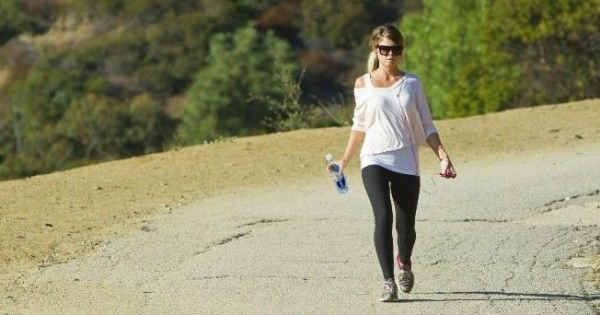
\includegraphics[width=0.4\textwidth]{figures/ssd1_coco}} \hspace{10pt}
	\subfigure[]{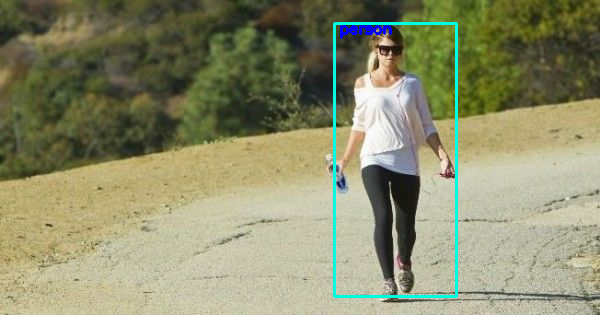
\includegraphics[width=0.4\textwidth]{figures/ssd1_voc}}
	\subfigure[]{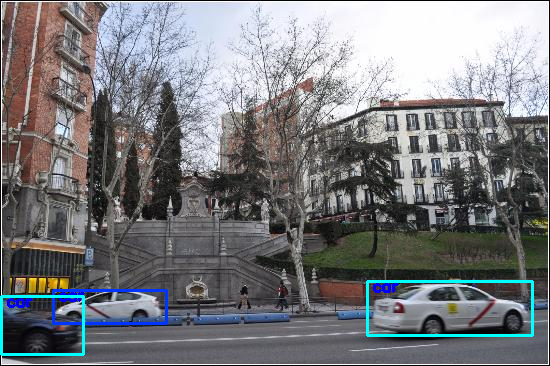
\includegraphics[width=0.4\textwidth]{figures/ssd2_coco}} \hspace{10pt}
	\subfigure[]{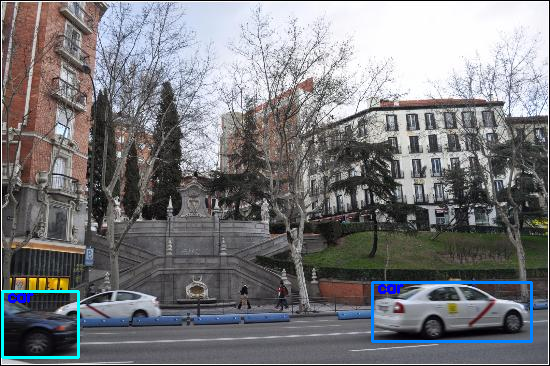
\includegraphics[width=0.4\textwidth]{figures/ssd2_voc}}
	\subfigure[]{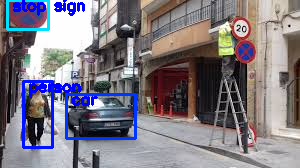
\includegraphics[width=0.4\textwidth]{figures/ssd3_coco}} \hspace{10pt}
	\subfigure[]{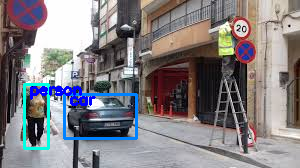
\includegraphics[width=0.4\textwidth]{figures/ssd3_voc}}
	\caption{Detección en distintas imágenes: (a)~Imagen sencilla con \acrshort{coco}, (b)~Imagen sencilla con \acrshort{voc}, (c)~Imagen complejo con \acrshort{coco}, (d)~Imagen compleja con \acrshort{voc}, (e)~Señal de tráfico con \acrshort{coco}, (f)~Señal de tráfico con \acrshort{voc}}
	\label{fig.ssd1}
\end{figure}

En una imagen bastante sencilla~(a) y~(b), el modelo de \textit{Pascal \acrshort{voc}} es capaz de detectar a la persona, mientras que el modelo \acrshort{coco} no la detecta. Por el contrario, en un escenario un poco más complicado~(c) y~(d), el modelo \acrshort{voc} no detecta uno de los coches de la escena, mientras que el modelo \acrshort{coco} realiza la detección de todos los coches. Por último, en las imágenes~(e) y~(f), la señal que aparece en primer plano queda identificada por \acrshort{coco}, pues entre sus etiquetas se incluyen este tipo de objetos, pero no por \acrshort{voc}, pues no incluyen etiquetas de este estilo.\\

Para tratar de obtener algún resultado concluyente se introdujo en la red una serie de imágenes de grises. Puesto que la red está entrenada con imágenes de color RGB será necesario replicar la propia imagen en las tres componentes para hacer coincidir las dimensiones de las imágenes y realizar la detección. En la Figura~\ref{fig.ssd2} se muestra cómo, con el modelo \acrshort{coco}~(a) y~(b), al realizar la detección en una imagen de grises, cuyo resultado en color era correcto para la persona a pesar de no detectar la bicicleta, comete un error a la hora de indicar la etiqueta de uno de los objetos detectados, equivocando la bicicleta con una persona. En el caso del modelo \acrshort{voc}~(c) y~(d) de la Figura~\ref{fig.ssd2}, se puede comprobar cómo se detecta un mayor número de personas al utilizar la imagen de grises que al emplear la imagen RGB.
\begin{figure}[H]
	\centering
	\subfigure[]{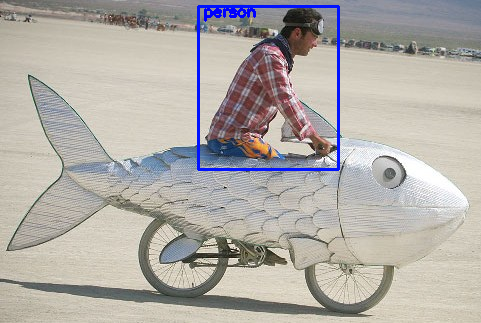
\includegraphics[width=0.4\textwidth]{figures/ssd4_color}} \hspace{10pt}
	\subfigure[]{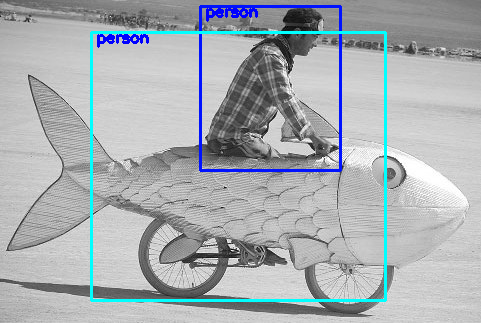
\includegraphics[width=0.4\textwidth]{figures/ssd4_gris}}
	\subfigure[]{\includegraphics[width=0.4\textwidth]{figures/ssd5_color}} \hspace{10pt}
	\subfigure[]{\includegraphics[width=0.4\textwidth]{figures/ssd5_gris}}
	\caption{Detección en distintas imágenes: (a)~Imagen RGB con \acrshort{coco}, (b)~Imagen de grises con \acrshort{coco}, (c)~Imagen RGB con \acrshort{voc}, (d)~Imagen de grises con \acrshort{voc},}
	\label{fig.ssd2}
\end{figure}

Se puede decir que la resolución del problema de detección con los ejemplos proporcionados por Caffe resulta bastante satisfactoria. Al introducir a la red imágenes escogidas de forma totalmente aleatoria se observan buenos resultados en la mayoría de los casos, pues se detectan correctamente un gran número de estímulos. Sin embargo, sobre qué red resulta mejor para la detección de un determinado estímulo no es posible establecer ninguna conclusión firme, pues es necesario un estudio más profundo.\\

Respecto a la importancia de la componente de color en la red entrenada, ocurre algo similar que en la comparación de ambas redes. Al introducir imágenes de grises en las redes entrenadas con color no existe ningún resultado que marque una evidencia sobre cómo de importante es esta componente en la detección. Es por esto que será necesario realizar un estudio más profundo de los modelos utilizados, con bases de datos de evaluación significativas, para obtener conclusiones sólidas sobre el enfoque \acrshort{ssd} de Caffe.\\

